\documentclass{beamer}
\usepackage{../common_slides}
\usepackage{tikz-qtree}

\title{Language Modeling \\ + \\ Feed-Forward Networks 3}
\date{}
\author{CS 287}

\usepackage{stackengine}
\stackMath
\newlength\matfield
\newlength\tmplength
\def\matscale{1.}
\newcommand\dimbox[3]{%
  \setlength\matfield{\matscale\baselineskip}%
  \setbox0=\hbox{\vphantom{X}\smash{#3}}%
  \setlength{\tmplength}{#1\matfield-\ht0-\dp0}%
  \fboxrule=1pt\fboxsep=-\fboxrule\relax%
  \fbox{\makebox[#2\matfield]{\addstackgap[.5\tmplength]{\box0}}}%
}
\newcommand\raiserows[2]{%
   \setlength\matfield{\matscale\baselineskip}%
   \raisebox{#1\matfield}{#2}%
}
\newcommand\matbox[4]{
  \stackunder{\dimbox{#1}{#2}{$#4$}}{\scriptstyle #3}%
}

\begin{document}

\begin{frame}
  \titlepage
\end{frame}

\begin{frame}{Review: LM ML Setup}

  Multi-class prediction problem, 

  \[ (\boldx_1, \boldy_1), \ldots, (\boldx_n, \boldy_n) \]
  \begin{itemize}
  \item $\boldy_i$; the one-hot next word
  \item $\boldx_i$; representation of the prefix $(w_1, \ldots, w_{t-1})$
  \end{itemize}

  \textbf{Challenges:}
  \begin{itemize}
  \item How do you represent input?
  \item Smoothing is crucially important.
  \item Output space is very large (next class)
  \end{itemize}
\end{frame}

\begin{frame}{Review: Perplexity}
  Previously, used \textit{accuracy} as a metric.
  
  \air 

  Language modeling uses of version  average negative
  log-likelihood 
  \begin{itemize}
    \item For test data $\bar{w}_1, \ldots, \bar{w}_n$
    \item \[NLL = -\frac{1}{n}\sum_{i=1}^n \log p(w_i | w_1, \ldots,w_{i-1})\]
  \end{itemize}


  Actually report \textit{perplexity},
  \[ perp = \exp(-\frac{1}{n}\sum_{i=1}^n \log p(w_i | w_1, \ldots,w_{i-1})) \]

  Requires modeling full distribution as opposed to argmax (hinge-loss)
\end{frame}

\begin{frame}{Review: Interpolation (Jelinek-Mercer Smoothing)}
  Can write recursively,

  \[ p_{interp}(w |  c) =  \lambda p_{ML}(w |  c) + (1 - \lambda) p_{interp}(w | c') \]

  Ensure that $\lambda$ form convex combination
  \[0 \leq \lambda \leq 1\]

  How do you learn conjunction combinations?
\end{frame}


\begin{frame}{Quiz}
  % We talked briefly last class about using language models for smoothing. 
  % It has become a popular task in recent years to utilize language models to predict 
  % missing words, for example consider the Microsoft Research Sentence Completion Challenge.
  Assume we have seen the following training sentences, 

  \begin{itemize}
  \item     a tractor drove slow
  \item     the red tractor drove fast
  \item     the parrot flew fast

  \item the parrot flew slow
    
    \item the tractor slowed down

  \end{itemize}


  Compute $p_{ML}$ for bigrams and use them to estimate whether \textit{parrot} or \textit{tractor}  fit better in the following contexts.


  \begin{enumerate}
    \item the  red \_\_\_ ?
    \item the  \_\_\_ ?

    \item the  \_\_\_ drove?
  \end{enumerate}

\end{frame}



\begin{frame}[allowframebreaks]{Answer}
  \begin{table}
    \centering
    \begin{tabular}{lll}
      \toprule
      \midrule
      a & tractor & 1\\
      \midrule
      the & red & $\frac{1}{4}$\\
      the & parrot & $\frac{1}{2}$\\
      the & tractor &$\frac{1}{4}$ \\
      \midrule
      red & tractor & 1 \\
      \midrule
      tractor & drove & $\frac{2}{3}$ \\
      tractor & slowed & $\frac{1}{3}$ \\
      \midrule
      parrot & flew & 1 \\
      $\ldots$ & & \\
      \bottomrule
    \end{tabular}
  \end{table}

\newpage
  \begin{itemize}
  \item the red tractor 
  \item the parrot 
  \item the tractor drove 
  \end{itemize}
  

\end{frame}


\begin{frame}{Today's Class }
  \[ p(w_i | w_{i-n+1}, \ldots w_{i-1}; \theta) \] 

  \begin{itemize}
  \item Estimate this directly as a neural network.
    \air 

  \item Two types of models, neural network and log-bilinear. 
    \air 

  \item Efficient methods for approximated estimation.
  \end{itemize}
\end{frame}


\begin{frame}{Intuition: NGram Issues}
  
  In training we might see, 

  \begin{center}
    the arizona corporations commission \alert{authorized}
  \end{center}

  But at test we see, 
  \begin{center}
    the colorado businesses organization \alert{\_\_\_}
  \end{center}
  \pause 
  
  \begin{itemize}
  \item Does this training example help here?
    \begin{itemize}
    \item Not really. No count overlap.
    \end{itemize}
    \air 
    \pause 
  \item Does backoff help here? 
    \begin{itemize}
    \item Maybe, if we have seen organization.
    \item Mostly get nothing from the earlier words.
    \end{itemize}
  \end{itemize}
\end{frame}


\begin{frame}{Goal}
  \begin{itemize}
  \item Learn representations that share properties between similar words.

    \air
  \item Particularly helpful for unseen contexts.


   \air 

  \item Not a silver bullet, e.g. proper nouns



  \begin{center}
    the eagles play the arizona \alert{diamondbacks}
  \end{center}

  Whereas at test we might see, 

  \begin{center}
    the eagles play the colorado  \alert{\_\_\_}
  \end{center}  
  (We will discuss this issue more for in MT)
  \end{itemize}
\end{frame}



\begin{frame}{Baseline: Class-Based Language Models}
  \begin{itemize}
  \item Groups words into classes based on word-context.
  \begin{center}
    \Tree [ $\ldots$ [ .3 dog cat horse $\ldots$ ] $\ldots$ [ .5 car
    truck motorcycle $\ldots$ ] ]
  \end{center}
  \item Various factorization methods for estimating with count-based approaches.
    \air 
  \item However, assumes a hard-clustering, often estimated separately.
  \end{itemize}
\end{frame}



\section{Neural Language Models}

\begin{frame}{Recall: Word Embeddings}
  \begin{itemize}
  \item Embeddings give multi-dimensional representation of words. 

    \item Ex: Closest by cosine similarity

      \begin{small}
        \begin{center}
          arizona
          \begin{tabular}{ll}
            texas& 0.932968706025 \\
            florida & 0.932696958878\\
            kansas&0.914805968271\\
            colorado&0.904197441085\\
            minnesota&0.863925347525\\
            carolina&0.862697751337\\
            utah& 0.861915722889\\
            miami&0.842350326527\\
            oregon&0.842065064748\\
          \end{tabular}
        \end{center}
      \end{small}
    \item Gives a multi-clustering over words. 
  \end{itemize}
  % corporations
  % \begin{tabular}{ll}
  % firms& 0.894882639809\\
  % companies&0.86738377358\\
  % businesses&0.859315950927\\
  % corporate&0.821590295322\\
  % enterprises&0.818504805202\\
  % investing&0.765133327454\\
  % institutions&0.76372338938\\
  % subsidiaries&0.762939166391\\
  % lobbyists&0.759909805468\\
  % \end{tabular}
\end{frame}


\begin{frame}{Feed-Forward Neural NNLM (Bengio, 2003)}
  \begin{itemize}

  \item $w_{i-n+1},\ldots w_{i-1}$ are input embedding representations
    \air 

  \item $w_i$ is an output embedded representation
    \air

  \item Model simultaneously learns,
    \begin{itemize}
    \item input word representations
      \air 
    \item output word representations
      \air 
    \item conjunctions of input words (through NLM, no n-gram features)
    \end{itemize}
  \end{itemize}
\end{frame}


\begin{frame}{Feed-Forward Neural Representation}
  \begin{itemize}
  \item $p(w_i | w_{i-n+1}, \ldots w_{i-1}; \btheta)$
  \item $f_1, \ldots, f_{\dwin}$ are words in window
  \item Input representation is the concatenation of embeddings
  \end{itemize}

  \[ \boldx = [v(f_1)\  v(f_2) \  \ldots \  v(f_{\dwin})]  \]

  Example: NNLM ($\dwin = 5$)
  \[ [\textcolor{blue}{w_3\ w_4\ w_5\ w_6\ w_7}]\ \textcolor{red}{w_8} \]
  \[ \boldx = [v(w_3)\  v(w_4) \  v(w_5) \ v(w_6) \ v(w_7)]  \]

  \[\renewcommand\matscale{.6}
\matbox{1.5}{4}{\din /5}{} \matbox{1.5}{4}{\din /5}{} \matbox{1.5}{4}{\din /5}{\boldx} \matbox{1.5}{4}{\din /5}{} \matbox{1.5}{4}{\din /5}{}% \raiserows{1.5}{\matbox{4}{2}{d_0}{\dout}{\boldW^0}}  \matbox{4}{2}{\din}{\dout}{\boldW^1} +
% \matbox{7}{2}{1}{\dout}{\boldb}
\]

  
\end{frame}


\begin{frame}{A Neural Probabilistic Language Model (Bengio, 2003)}  
  One hidden layer multi-layer perceptron architecture,

  \[NN_{MLP1}(\boldx) =  \tanh(\boldx\boldW^1 + \boldb^1)\boldW^2 + \boldb^2\]
  
  Neural network architecture on top of concat.

  \[\hat{\boldy} = \softmax(NN_{MLP1}(\boldx)) \] 
%  \iar 
%
  Best model uses $\din=30 \times \dwin, \dhid =100$.
%
\end{frame}

\begin{frame}{A Neural Probabilistic Language Model }  
  Optional, direct connection layers,

  \[NN_{DMLP1}(\boldx) =  [\tanh(\boldx\boldW^1 + \boldb^1), \boldx] W^2 + \boldb^2\]

  \begin{itemize}
  \item $\boldW^1 \in \reals^{\din \times \dhid}, \boldb^1 \in \reals^{1 \times \dhid}$; first affine transformation
  \item $\boldW^2 \in \reals^{(\dhid + \din)  \times \dout}, \boldb^2 \in \reals^{1 \times \dout}$; second affine transformation
  \end{itemize}
\end{frame}

\begin{frame}{A Neural Probabilistic Language Model (Bengio, 2003)}  
  \begin{center}
    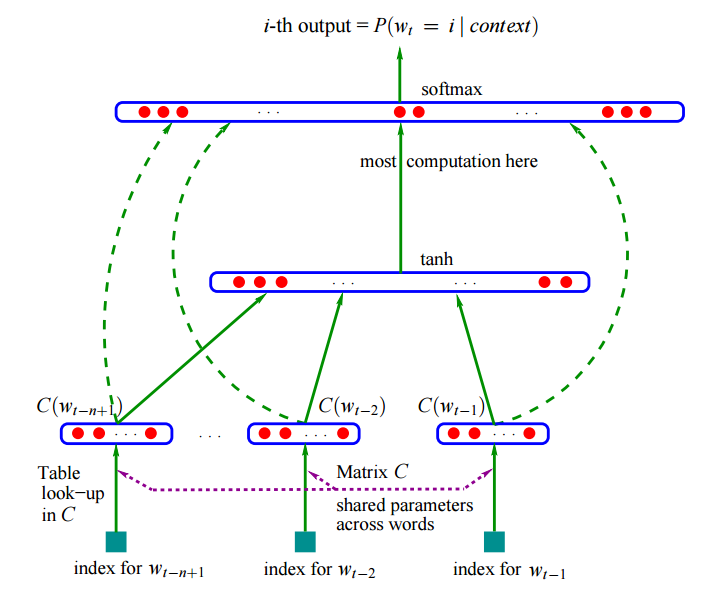
\includegraphics[width=7cm]{bengio}
  \end{center}
  Dashed-lines show the optional direct connections, $C = v$.
\end{frame}



\begin{frame}{A Neural Probabilistic Language Model }  
  \begin{center}
    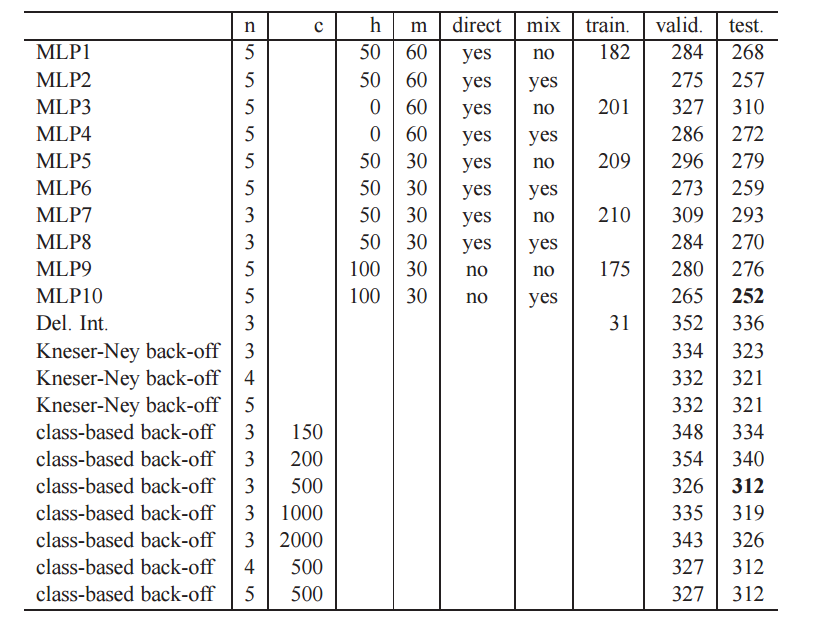
\includegraphics[width=9cm]{bengioresults}
  \end{center}
\end{frame}

\begin{frame}{Parameters}
  \begin{itemize}
  \item Bengio NNLM has $\dhid=100$, $\dwin=5$, $\din = 5 \times 50 $ 
    \air 
    
  \item In-Class: How many parameters does it have? How does this compare to Kneser-Ney smoothing?
  \end{itemize}
\end{frame}

\begin{frame}{Historical Note}
  \begin{itemize}
  \item Bengio et al notes that many of these aspects predate the work
    \air 
  \item Furthermore proposes many of the ideas that Collobert et al. and word2vec implement and scale 
    \air 
  \item Around this time, very few NLP papers on  NN, most-cited papers are about conditional random fields (CRFs). 
  \end{itemize}
\end{frame}


\begin{frame}{Log-Bilinear Language Model (Mnih \& Hinton, 2007)}

Slightly different input representation. Now let:

\[ \boldx = \sum_{i=1}^{\dwin} v(f_i) \boldC_i \]

\begin{itemize}
\item Instead of concatenating, weight each $v(f_i)$ by position-specific weight matrix $\boldC_i$.
\end{itemize}

Then use:

  \[\hat{\boldy} = \softmax(\boldx\boldW^1 + \boldb)\]

  \begin{itemize}
  \item Note no tanh layer.
  %  \air 
  \item $\boldW^1$ can use input embeddings too, or not (Mnih and Teh, 2012)
  \item Can be faster to use, and in some cases simpler.
  \end{itemize}
\end{frame}



\begin{frame}{Comparison}
  Both count-based models and feed-forward NNLMs are Markovian language models, 

  Comparison:
  \begin{itemize}
  \item Training Speed: ngrams are much faster (more coming)
  \item Usage Speed: ngrams very fast, NN can be fast with some tricks. 
  \item Memory: NN models can be much smaller (but there are big ones)
  \item Accuracy: Comparable for small data, NN does better with more.
  \end{itemize}
  
  Advantages of NN model
  \begin{itemize}
  \item Can be trained end-to-end.
    \air 
  \item Does not require smoothing methods.
  \end{itemize}

  % \alert{NGram Models}
  % \begin{itemize}
  % \item Fast to train
  % \item Can 
  % \end{itemize}

  % \structure{Neural Models}
  % \begin{itemize}
  % \item Slower to train
  % \item
  % \end{itemize}
\end{frame}

\begin{frame}{Translation Performance ( and Blunsom, 2015)}
  \begin{center}
    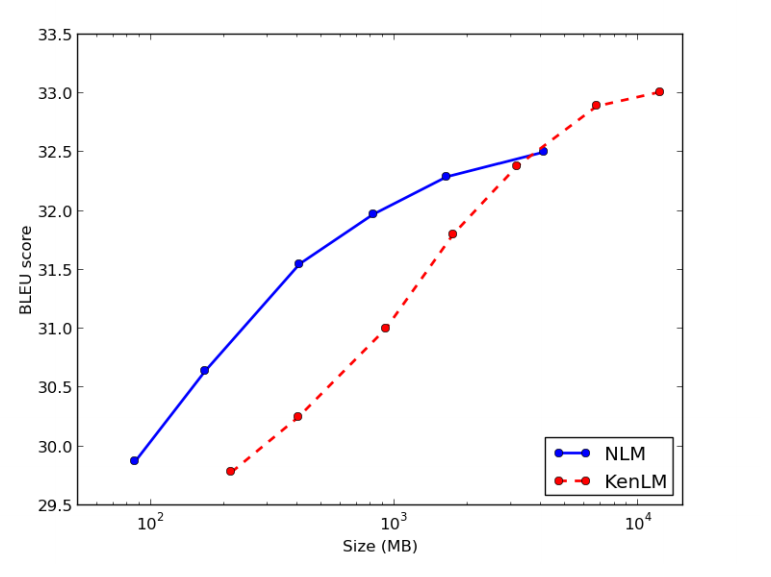
\includegraphics[width=8cm]{blunsomgraph}
  \end{center}
\end{frame}


\section{Noise Contrastive Estimation}

\begin{frame}{Review: Softmax Issues}
  Use a softmax to force a distribution,

  \[\softmax(\boldz) = \frac{\exp(\boldz)}{\displaystyle \sum_{w\in \mcC } \exp(z_w)}  \]

  \[\log \softmax(\boldz) = \boldz - \log \sum_{w\in \mcC} \exp(z_w)  \]

  \begin{itemize}
  \item \textbf{Issue:} class $\mcC$ is huge.
  \item For C\&W, 100,000, for word2vec 1,000,000 types
  \item Note largest dataset is 6 billion words
  \end{itemize}

\end{frame}



\begin{frame}{Unnormalized Scores}
  Recall the score defined as (dropping bias) 
  \[ \boldz = \tanh(\boldx \boldW^1)\boldW^2  \] 

  Unnormalized score of each word before soft-max, 

  \[ z_j = \tanh(\boldx \boldW^1)\boldW^2_{*,j}  \] 
  for any  $j \in \{1, \ldots \dout\}$
  \air 

  Note: can be computed efficiently $O(1)$ versus $O(\dout)$. 
\end{frame}


\begin{frame}{Coherence }
  \begin{itemize}
  \item Saw similar idea earlier for ranking embedding. 
    \air 

  \item \textbf{Idea:} Learn to distinguish coherent n-grams from 
    corruption. 
    \air 
 

    \air
  \item Want to discriminate correct next words from other choices.

    \begin{center}
      [ the dog \structure{walks} ]
    \end{center}
    
    
    

    \begin {center}
      [ the dog \alert{house}  ]
      
      [ the dog \alert{cats}  ]
      
      [ the dog \alert{skips}  ]
      
    \end{center}
  \end{itemize}
\end{frame}

\begin{frame}{Warm-Up}
 Imagine we have a new dataset, 
  \[ ((\boldx_1, \boldy_1), \boldd_1),\ldots, ((\boldx_n, \boldy_n), \boldd_n), \]
 
  \begin{itemize}
  \item $\boldx$; representation of context  $w_{i-n+1}, \ldots w_{i-1}$ 
  \item $\boldy$; a possible $w_i$
  \item $d$; 1 if $\boldy$ is correct, 0 otherwise
  \end{itemize}
  
  Objective is based on predicted $\hat{d}$:

  \[ \mathcal{L}(\theta) = \sum_{i} L_{crossentropy}(d_i, \hat{d}_i) \] 
\end{frame}


\begin{frame}{Warm-Up: Binary Classification}
  How do we score $(\boldx_i, \boldy_i = \bolddelta(w))$? 
\air 

Could use unnormalized score,
  \[ z_w = \tanh(\boldx \boldW^1)\boldW^2_{*,c}  \] 


  Becomes softmax regression/non-linear logistic regression,

  \[\hat{d} = \sigma(z_w)\]

  \begin{itemize}
  \item Much faster
  \item  But does not help us train LM.
  \end{itemize}

\end{frame}


\begin{frame}{Implementation}
  
  Standard MLP language model, (only takes in $\boldx$) 

  \[\boldx \Rightarrow \boldW^1 \Rightarrow \tanh \Rightarrow  \boldW^2 \Rightarrow \softmax\]



  Computing binary  (takes in $\boldx$ and $\boldy$) 
  \[\hat{d} = \sigma(z_w)\]

 \[\boldx \Rightarrow \boldW^1 \Rightarrow \tanh \Rightarrow
 \begin{matrix}
   \cdot \\ 
   \boldW^2_{*, w} \mathrm{(Lookup)}
 \end{matrix}
\Rightarrow \sigma\]
\end{frame}



\begin{frame}{Noise Contrastive Estimation 1}
  Probabilistic model,
  \begin{itemize}
  \item Introduce random variable $D$
  \item If $D=1$ produce true sample
  \item If $D=0$ produce sample from a noise distribution.
  \item Hyperparameter $K$ is ratio of noise
  \end{itemize}


  \[p(D=1) =   \frac{1}{K+1}\]

  \[p(D=0) = \frac{K}{K+1}\]
   
\end{frame}

\begin{frame}{Noise Contrastive Estimation 2}

  For a given $\boldx, \boldy$, 
  \begin{eqnarray*}
  p(D=1 | \boldx, \boldy) &=&  \frac{p(\boldy|D=1, \boldx) p(D=1 | \boldx)}{\sum_{d} p(\ \boldy|D=d, \boldx ) p(D=d | \boldx) } \\
  &=&  \frac{p( \boldy|D=1, \boldx) p(D=1 | \boldx)}{p(\boldx|D=0)p(D=0 | \boldx) +  p(\boldy|D=1,\boldx)  p(D=1 | \boldx) }
  \end{eqnarray*}
  Plug-in the noise distribution and hyperparameters,
  \begin{eqnarray*}
    p(D=1 | \boldx, \boldy) &=& \frac{\frac{1}{K+1} p(\boldy|D=1, \boldx)}{\frac{1}{K+1} p(\boldy|D=1, \boldx) + \frac{K}{K+1} p(\boldy|D=0, \boldx) }\\
    &=& \frac{p(\boldy|D=1, \boldx)}{p(\boldy|D=1, \boldx) + K p(\boldy|D=0, \boldx) } \\
    &=& \sigma(\log p(\boldy|D=1, \boldx) - \log(K p(\boldy|D=0, \boldx))) \\  
  \end{eqnarray*}
\end{frame}


\begin{frame}{Noise Contrastive Estimation 3}
 With \[p(D=1 | \boldx, \boldy) = \sigma(\log p(\boldy|D=1, \boldx) - \log(K p(\boldy|D=0, \boldx)))\]
 
 we the training objective for a corpus that has $K$ noise samples $s_{i,k}$ per example is:
 
   \begin{align*}
\mathcal{L}(\theta) &= \sum_{i} \log p(D=1| \boldx_i, \boldy_i) + \sum_{k=1}^{K} \log p(D=0|\boldx_i, Y=s_{i,k})  \\
&= \sum_{i} \log \sigma\left(\log p(\boldy_i|D=1, \boldx_i) - \log(K p(\boldy_i|D=0, \boldx_i))\right) \\
& + \sum_{k=1}^{K} \log \left(1 - \sigma\left(\log p(s_{i,k}|D=1, \boldx_i) - \log(K p(s_{i,k}|D=0, \boldx_i))\right)\right)
\end{align*}
%   &=& \sum_{i} \log \sigma(\hat{z}_c - \log(K p_{ML}(c))) \\
% &+&   \sum_{k=1}^{K} \log (1- \sigma(\hat{z}_{s_{i,k}} - \log(K p_{ML}(s_{i,k}))))  
% \end{eqnarray*}

  \begin{itemize}
%  \item   $s_{i,k}$ are $K$ samples for each position $i$   
%  \end{itemize}
  
%  \begin{itemize}
%  \item $\log p(\boldy=c|D=1, \boldx)$; becomes $z_c$ (as above)
%    \air
%  \item $\log p(\boldy=c|D=0, \boldx)$; noise distribution 
%    \air 
  \item In practice, sample $s_{i,k}$ from unigram distribution 
%    \air 
%
%  \item (Can precompute samples and noise scores)
  \end{itemize}
\end{frame}

\begin{frame}{Noise Contrastive Estimation 4}
But we still have a problem: $\mathcal{L}$ defined in terms of normalized distributions $\log p(\boldy|D=1, \boldx)$

\textbf{Solution:} 
\begin{itemize}
\item instead of explicitly normalizing, estimate $Z({\boldx})$, normalizing constant of each context $\boldx$, \textit{as a parameter} (Gutmann \& Hyv{\"a}rinen, 2010)
\item  Mnih and Teh (2012) show that fixing $Z({\boldx})=1$ for all contexts works just as well
\item So we can replace $\log p(\boldy = \bolddelta(w)|D=1, \boldx)$ with $z_w$, as computed by our network
\end{itemize}

%  \[p(D=1 | \boldx, \boldy) = \sigma(\log p(\boldy|D=1, \boldx) - \log(K p(\boldy|D=0, \boldx)))\]
%
%  \begin{itemize}
%  \item $\log p(\boldy=c|D=1, \boldx)$; becomes $z_c$ (as above)
%    \air
%  \item $\log p(\boldy=c|D=0, \boldx)$; noise distribution 
%    \air 
%  \item In practice, people use unigram for noise
%    \air 
%
%  \item (Can precompute samples and noise scores)
%  \end{itemize}
\end{frame}


%\begin{frame}{Noise Contrastive Estimation 3}
%  \[p(D=1 | \boldx, \boldy) = \sigma(\log p(\boldy|D=1, \boldx) - \log(K p(\boldy|D=0, \boldx)))\]
%
%  \begin{itemize}
%  \item $\log p(\boldy=c|D=1, \boldx)$; becomes $z_c$ (as above)
%    \air
%  \item $\log p(\boldy=c|D=0, \boldx)$; noise distribution 
%    \air 
%  \item In practice, people use unigram for noise
%    \air 
%
%  \item (Can precompute samples and noise scores)
%  \end{itemize}
%\end{frame}

\begin{frame}{Noise Contrastive Estimation 5}
%
%  Full objective, 
%
%  \begin{itemize}
%  \item   $s_{i,k}$ are $K$ samples for each position $i$   
%  \end{itemize}
So we now have
  
  \begin{eqnarray*}
\mathcal{L}(\theta)
   &=& \sum_{i} \log \sigma(z_{w_i} - \log(K p_{ML}(w_i))) \\
 &+&   \sum_{k=1}^{K} \log (1- \sigma(z_{s_{i,k}} - \log(K p_{ML}(s_{i,k}))))  
 \end{eqnarray*}
 
 \begin{itemize}
 \item Mnih and Teh (2012) show that gradient of $\mathcal{L}$ approaches gradient of true language model's log-likelihood objective as $k \rightarrow \infty$.
% this yields a consistent estimation of the true LM distribution 
 \end{itemize}
\end{frame}

\begin{frame}{Implementation}
  \begin{itemize}
  \item How do you efficiently compute $z_w$?

    Need a lookup table (and dot-product) for output embeddings! (Not full matrix-vector product).

  \item How do you efficiently handle $\log p_{ML}(w)$
  
    Can be precomputed or placed in a lookuptable .

  \item How do you handle sampling?

    Can precompute large number of samples (not example specific).

    \item How do you handle loss?

    Simply BinaryNLL Objective.
  \end{itemize}
\end{frame}

\begin{frame}{Implementation}
  
  Standard MLP language model,

  \[\boldx \Rightarrow \boldW^1 \Rightarrow \tanh \Rightarrow  \boldW^2 \Rightarrow \softmax\]



  Computing $\sigma(z_w - \log(K p_{ML}(w)))$,
 \[\boldx \Rightarrow \boldW^1 \Rightarrow \tanh \Rightarrow
 \begin{matrix}
   \cdot \\ 
   \boldW^2_{*, w} \mathrm{(Lookup)}
 \end{matrix}
 \Rightarrow  \begin{matrix}
   - \\ 
   \log K p_{ML}(w) \mathrm{(input)}
 \end{matrix}
\Rightarrow \sigma\]


 %  $\boldx$ $\Rightarrow$ linear $\Rightarrow$ tanh  $\Rightarrow$\begin{tabular}{l} Dotproduct & LookupTable ($W_{}$)\end{tabular}
 % $\Rightarrow $ \begin{tabular}{l} Add \\ LookupTable (P(w))\end{tabular} $\Rightarrow$ Sigma
 
                                                                                       
  % \Tree [ .LookupTable [ .Linear [ .tanh [ .DotProduct(with w) [ .Subtract (log P(w))  .Sigma ]     ]  ]  ] ] ;   

  (Efficiency, compute first three layers only once for $K+1$)
  \air 
  
\end{frame}

\begin{frame}{Using in Practice}
  
  Several options for test time,
  \begin{itemize}
  \item Use full softmax with learned parameters.
    \air 
  \item Compute subset of scores and renormalize (homework)
.
\air 

\item Can sometimes just use treat unormalized params as being normalized (self-normalization)
  \end{itemize}


\end{frame}

% \begin{frame}{Noise Distribution}
%   What noise distribution should you use.

%   Unigram estimations.
% \end{frame}


% \begin{frame}{Use as an LM}
%   \begin{itemize}
%   \item Unlike HSM learns full $\boldW^2$ 
%     \air 

%   \item Can run $\softmax(tanh(\boldx \boldW^1) + \boldW^2)$ at test time. 

%   \item Instead of 1 multiclass, we do 1+K binary classifications


%   \end{itemize}
% \end{frame}

% \% begin{frame}{Comparison With }
%   \begin{itemize}
%   \item 
%   \item 
%   \end{itemize}
% \end{frame}

% \begin{frame}{Loss Criterions}

%   \begin{center}

%   \begin{tikzpicture}
%     \node(x)[text width=3cm,text centered]{prediction\\ $\hat{\boldY} $};
%     \node(t)[text  width=3cm,text centered, below right= of x, draw]{  $L(*, *)$};

%     \node(fx)[text width=3cm,text centered, above right=of t]{loss\\$L(\boldY, \hat{\boldY})$};
%     \node(gradin)[text width=3cm,text centered, below left =of t]{self.gradInput\\ $\displaystyle \frac{\partial L}{\partial \hat{\boldY} } $};
%     \node(gradout)[text width=3cm,text centered, below right= of t]{target \\ $\boldY$   };
%     % \node(gradweight)[text width=3cm,text centered, below = of t]{self.gradWeight\\ $\displaystyle  \frac{\partial L}{\partial \btheta_{i+1}  }$};

%     \path[text width=3cm,text centered, draw, ->] (x) -> (t);
%     \path[text width=3cm,text centered, draw, ->] (t) -> (fx);
%     \path[text width=3cm,text centered, draw, ->] (t) -> (gradin);
%     \path[text width=3cm,text centered, draw, ->]  (gradout) -> (t);
%   \end{tikzpicture}
%   \end{center}
% \end{frame}


\end{document}